\section{Holographic Projection}
\label{sec.holographic_projection}

In the proposed holographic projection, the perspective projection is computed in a similar way, a 3D point in a truncated pyramid frustum (eye coordinates) is mapped to NDC; and the range of $x$ and $y$-coordinates from respectively $[l, r]$ and $[b, t]$ are still  mapped to $[-1, 1]$, but the $z$-coordinate is mapped in the inverse way, from $[n, f]$ to $[1, -1]$. 

Note that the eye coordinates are still defined in the right-handed coordinate system, but now the camera at the origin is looking along $+Z$ axis in eye space, but it is looking along $+Z$ axis in NDC. This inversion in the orientation of the $Z$ axis can be achieve by a permutation matrix, which changes the orientation of the $z$ coordinates and negates the third column of the projection matrix in Equation~\ref{eq.projection_matrix}.

%Since glFrustum() accepts only positive values of near and far distances, we need to negate them during the construction of \verb|GL_PROJECTION| matrix.

\begin{figure}[h!]
\centering
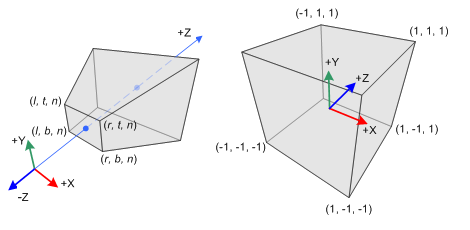
\includegraphics[width=0.9\linewidth,keepaspectratio=true]{figs/new_gl_projectionmatrix01.png}
\caption{Perspective Frustum and Normalized Device Coordinates (NDC)}
\label{fig.new_projection01}
\end{figure}


%The following diagrams show how a point $(x_e, y_e, z_e)$ in eye space is projected to $(x_p, y_p, z_p)$ on the near plane.

%\begin{figure}[!ht]
%\centering
%\begin{tabular}{cc}
%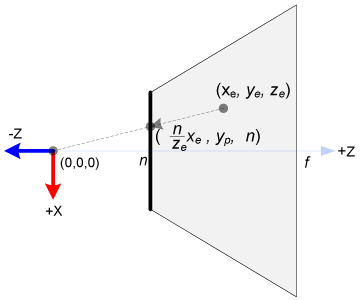
\includegraphics[width=0.45\linewidth,keepaspectratio=true]{figs/new_gl_projectionmatrix03.png}&
%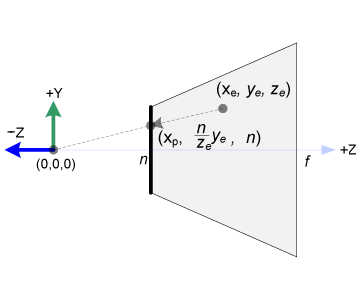
\includegraphics[width=0.45\linewidth,keepaspectratio=true]{figs/new_gl_projectionmatrix04.png}\\
%Top View of Frustum&
%Side View of Frustum
%\end{tabular}
%\caption{Views of the frustum.}
%\label{fig.new_frustum}
%\end{figure}

The permuted projection matrix is; 
\begin{equation}
\begin{aligned}
\begin{pmatrix} x_{c}\\y_{c}\\z_{c}\\w_{c} \end{pmatrix} &= 
\begin{pmatrix} 
\frac{2n}{r-l} & 0 & -\frac{r+l}{r-l} & 0 \\
0 & \frac{2n}{t-b} & -\frac{t+b}{t-b} & 0 \\
\cdot & \cdot & -\frac{(f+n)}{f-n} & \frac{2fn}{f-n} \\
0 & 0 & 1 & 0 \\
\end{pmatrix} \\
\end{aligned}
\end{equation}

